\documentclass[10pt,a4paper,titlepage]{report}
\usepackage[utf8]{inputenc}
\usepackage{amsmath}
\usepackage{amsfonts}
\usepackage{amssymb}
\usepackage{graphicx}
\usepackage{xcolor}
\usepackage{minted}


\nonstopmode
\begin{document}
\begin{titlepage}
\author{Rwithik Manoj}
\title{Awk Scripting}
\date{\today}
\maketitle
\end{titlepage}

\begin{enumerate}
	\item Write a awk script that accepts date argument in the form of mm-dd-yy and displays it in the following format. The script should check the validity of the argument and in the case of error, display a suitable message.\newline
	\textbf{Algorithm:}\newline
	\begin{enumerate}
			\item Start.
			\item Check if the date is valid. Exit if its not. 
			\item If it is a valid date, find the corrosponding month. And print the output in the format specified.
			\item Stop.
	\end{enumerate}
	\textbf{Script:}\newline
	\inputminted[tabsize=4]{awk}{../Scripts/Awk/1.awk}
	\textbf{Output:}\newline\newline
	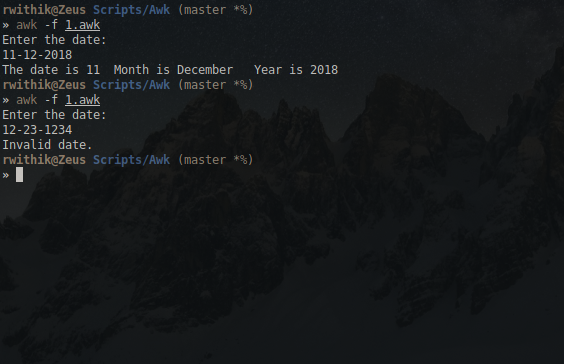
\includegraphics[width=\linewidth]{../Images/Awk/1.png}
	\item Write an awk script to delete duplicated line from a text file. The order of the original lines must remain unchanged.\newline
	\textbf{Algorithm:}\newline
	\begin{enumerate}
			\item Start.
			\item Print the line only if seen[\$0] is zero, ie the count of the current line is zero.
			\item Stop.
	\end{enumerate}
	\textbf{Script:}\newline
	\inputminted[tabsize=4]{awk}{../Scripts/Awk/2.awk}
	\textbf{Output:}\newline\newline
	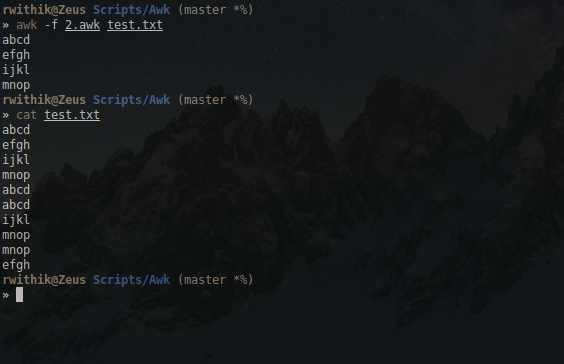
\includegraphics[width=\linewidth]{../Images/Awk/2.png}
	\item Write an awk script to find out total number of books sold in each discipline as well as total book sold based on the given table.\newline
	\textbf{Algorithm:}\newline
	\begin{enumerate}
			\item Start.
			\item Initalise sum to 0.
			\item Add the second field to the sum.
			\item Add the Second field to the corrosponding array element.
			\item Print the values.
			\item Stop.
	\end{enumerate}
	\textbf{Script:}\newline
	\inputminted[tabsize=4]{awk}{../Scripts/Awk/3.awk}
	\textbf{Output:}\newline\newline
	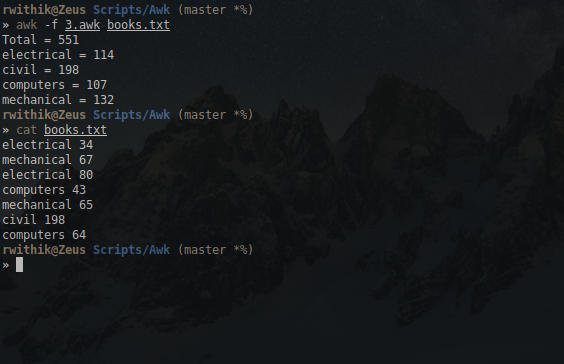
\includegraphics[width=\linewidth]{../Images/Awk/3.png}
	\item Write an awk script to compute gross salary of an employee accordingly to rule given below: If basic salary is less than 10000, then DA = 45\% of the basic and HRA = 15\% of basic. If basic salary is greater than 10000, then DA = 50\% of the basic and HRA = 20\% of basic.\newline
	\textbf{Algorithm:}\newline
	\begin{enumerate}
			\item Start.
			\item Check if the basic pay is less than 10000. If it is, calculate the total salary as BP + 0.45BP + 0.15BP.
			\item Otherwise, the total salary is BP + 0.5BP + 0.2BP.
			\item Stop.
	\end{enumerate}
	\textbf{Script:}\newline
	\inputminted[tabsize=4]{awk}{../Scripts/Awk/4.awk}
	\textbf{Output:}\newline\newline
	
\includegraphics[width=\linewidth]{../Images/Awk/4.png}
\end{enumerate}

\end{document}
